\chapter{Конструкторская часть}

В данном разделе будет рассмотрена общая архитектура приложения, алгоритм перехвата системных вызовов и подсчёт количества этих вызовов за выбранный промежуток времени.

\section{Архитектура приложения}

В состав разработанного программного обеспечения входит один загружаемый модуль ядра, который перехватывает все вызовы системных вызовов, подсчитывая их количество за определенный промежуток времени, предоставляет пользователю информацию о процессах и их состояниях, а так же информацию о состояние о загруженности оперативной памяти -- её общее количество, свободной и доступной в данный момент.

\section{Алгоритм перехвата системного вызова}

На риснуке \ref{fig:ftrace_algo} представлена схема алгоритма перехвата системных вызовов на примере \texttt{sys\_clone}.

\begin{figure}[h]
	\begin{center}
		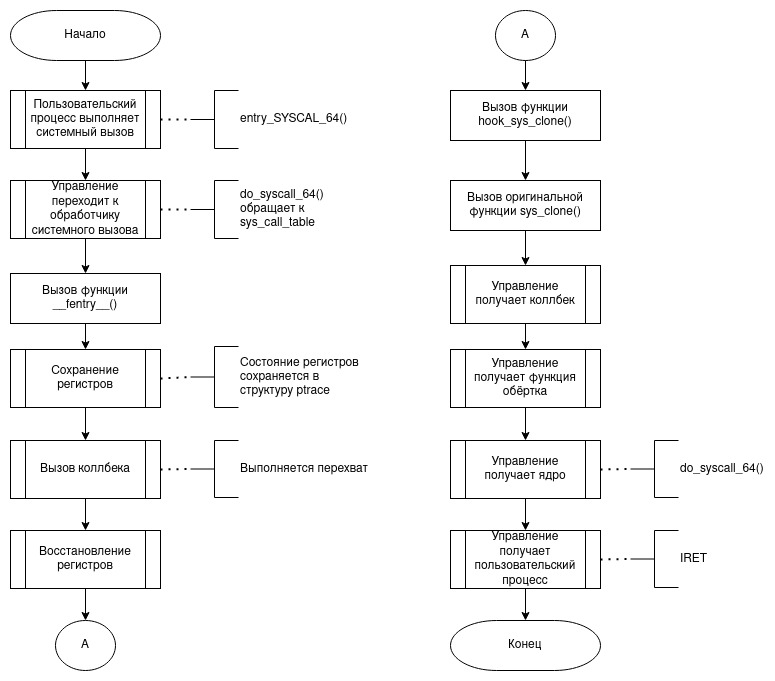
\includegraphics[scale=0.6]{img/ftrace_algo.jpg}
	\end{center}
	\caption{Алгоритм перехвата системного вызова}
	\label{fig:ftrace_algo}
\end{figure}

\begin{enumerate}
	\item Пользовательский процесс выполняет инструкцию \texttt{SYSCALL}. С помощью этой инструкции выполняется переход в режим ядра и управление передаётся низкоуровневому обработчику системных вызовов \texttt{entry\_SYSCALL\_64()}. Этот обработчик отвечает за все системные вызовы 64-битных программ на 64-битных машинах.
	
	\item Управление переходит к обработчику системного вызова. Ядро передаёт управление функции \texttt{do\_syscall\_64()}. Эта функция обращается к таблице обработчиков системных вызовов \texttt{sys\_call\_table} и с помощью неё вызывает конкретный обработчик системного вызова -- \texttt{sys\_clone()}.
	
	\item Вызывается \texttt{ftrace}. В начале каждой функции ядра находится вызов функции \texttt{\_\_fentry\_\_()}, реализованная фреймворком \texttt{ftrace}. Перед этим состояние регистров сохраняется в специальную структуру \texttt{pt\_regs}.
	
	\item \texttt{ftrace} вызывает разработанный коллбек.
	
	\item Коллбек выполняет перехват. Коллбек анализирует значение  \texttt{parent\_ip} и выполняет перехват, обновляя значение регистра \texttt{rip} (указатель на следующую исполняемую инструкцию) в структуре \texttt{pt\_regs}.
	
	\item \texttt{ftrace} восстанавливает значение регистров с помощью структуры \texttt{pt\_regs}. Так как обработчик изменяет значение регистр \texttt{rip} -- это приведёт к передачу управления по новому адресу.
	
	\item Управление получает функция обёртка. Благодаря безусловному переходу, управление получает наша функция \texttt{hook\_sys\_clone()}, а не оригинальная функция \texttt{sys\_clone()}. При этом всё остальное состояние процессора и памяти остаётся без изменений -- функция получает все аргументы оригинального обработчика и при завершении вернёт управление в функцию \texttt{do\_syscall\_64()}.
	
	\item Функция обёртка вызывает оригинальную функцию. \\Функция \texttt{hook\_sys\_clone()} может проанализировать аргументы и контекст системного вызова и запретить или разрешить процессу его выполнение. В случае его запрета, функция просто возвращает код ошибки. Иначе -- вызывает оригинальный обработчик \texttt{sys\_clone()} повторно, с помощью указателя \texttt{real\_sys\_clone}, который был сохранён при настройке перехвата.
	
	\item Управление получает коллбек. Как и при первом вызове \texttt{sys\_clone()}, управление проходит через \texttt{ftrace} и передается в коллбек.
	
	\item Коллбек ничего не делает. В этот раз функция \texttt{sys\_clone()} вызывается разработанной функцией \texttt{hook\_sys\_clone()}, а не ядром из функции \texttt{do\_syscall\_64()}. Коллбек не модифицирует регистры и выполнение функции \texttt{sys\_clone()} продолжается как обычно.
	
	\item Управление передаётся функции обёртке.
	
	\item Управление передаётся ядру. Функция \texttt{hook\_sys\_clone()} завершается и управление переходит к \texttt{do\_syscall\_64()}.
	
	\item Управление возвращает в пользовательский процесс. Ядро выполняет инструкцию \texttt{IRET}, устанавливая регистры для нового пользовательского процесса и переводя центральный процессор в режим исполнения пользовательского кода.
\end{enumerate}

\section{Алгоритм подсчёта количества системных вызовов}

На риснуке \ref{fig:ftrace_cnt_algo} представлена схема алгоритма подсчёта системных вызовов.

\begin{figure}[h]
	\begin{center}
		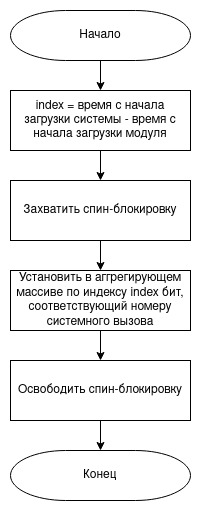
\includegraphics[scale=0.6]{img/ftrace_cnt_algo.jpg}
	\end{center}
	\caption{Алгоритм подсчёта количества системных вызовов}
	\label{fig:ftrace_cnt_algo}
\end{figure}

\begin{itemize}
	\item Аггрегирующий массив -- это массив на 86400 элементов, состоящий из структур, имеющих два поля в виде 64-битных беззнаковых целых чисел. Это позволяет фиксировать до 128 системных вызов в секунду на протяжении 24 часов. Такой массив занимает всего лишь 1350 килобайт оперативной памяти;
	
	\item спин-блокировка необходима с той целью, что несколько системных вызовов могут быть вызываны в один и тот же момент времени -- в таком случае, без блокировки, аггрегирующий массив потеряет часть данных;
\end{itemize}

\section*{Вывод}

В данном разделе была рассмотрена общая архитектура приложения, алгоритм перехвата системных вызовов и подсчёта количества этих вызовов за выбранный промежуток.


